\subsection{Branches and Tags}

Technically Subversion does not introduce separate concepts for branches and tags. Both branches and tags are versioned directories under repository root. As result Translator performs theirs translation in similar way. There are differences at Git level only:
\begin{enumerate}
	\compactlist
	\item Addition.
	\begin{itemize}
		\item Creation of /branches/\emph{B} directory leads to creation of a new branch reference \emph{B}.
		\item Creation of /tags/\emph{T} directory leads to addition of corresponding Tag Object with name \emph{T}.
	\end{itemize}
	\item Modification.
	\begin{itemize}
		\item Change at /branches/\emph{B} directory leads to updating of corresponding branch reference \emph{B}.
		\item Change at /tags/\emph{T} directory leads to the removal of obsolete Tag Object with name \emph{T} and creation of new Tag Object with the same name for corresponding Commit Object.
	\end{itemize}
	\item Deletion.
	\begin{itemize}
		\item Removal of /branches/\emph{B} directory leads to removal of corresponding reference \emph{B} at Git repository, when
		\item Removal of /tags/\emph{T} directory leads to removal of corresponding Tag Object with name \emph{T}.
	\end{itemize}
\end{enumerate}

The same rules could be treated in opposite direction --- every change of Git branch or tag leads to corresponding change of Subversion branch or tag.

This and further chapters consider scenarios with branches only. But every scenario could be applied to tags with the rules above taken into account.

\subsubsection{Subversion Branch Creation}

There is a number of ways to create branch in Subversion.

\begin{enumerate}
\compactlist
\item Branch creation by copying, figure \ref{svn_branch_creation}.

\begin{figure}[!h]
\label{svn_branch_creation}
\centering
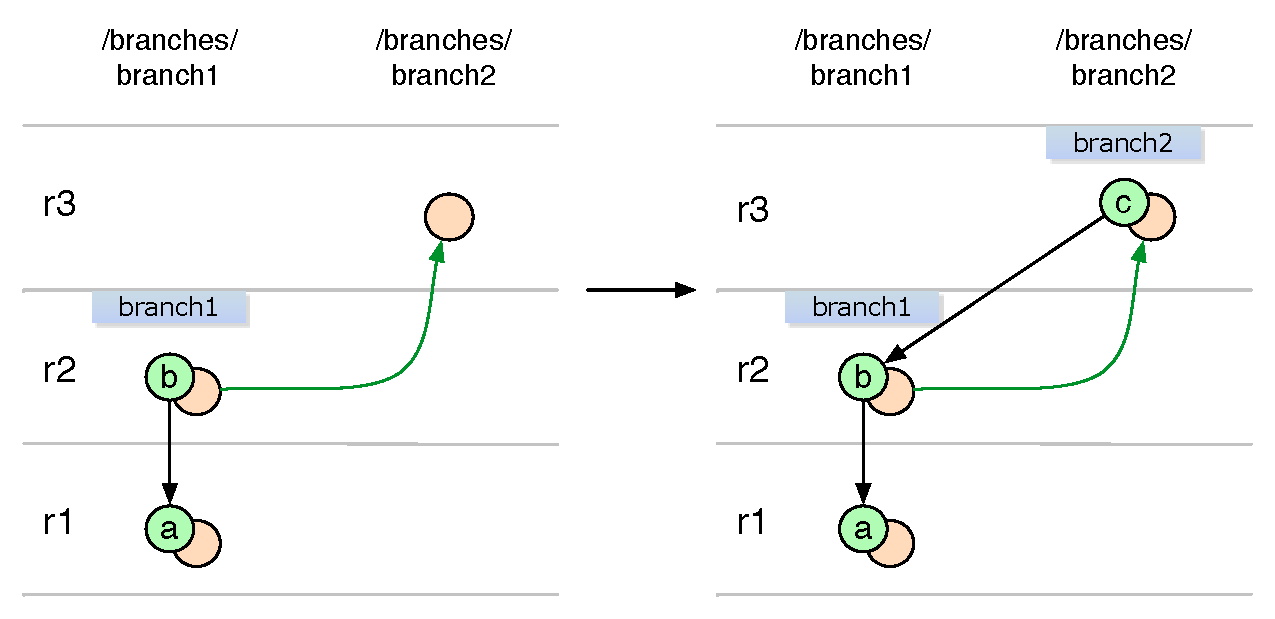
\includegraphics[width=\linewidth]{img/diagrams/branch_creation_svn_to_git.pdf}
\caption{Subversion branch copying being translated to Git branch creation.}
\end{figure}

Subversion user at revision r3 copied /branches/branch1@r2 to /branches/branch2. For that change Translator creates commit with:
\begin{itemize}
	\item Tree Object corresponding to /branches/branch2 subdirectory contents
	\item Author Ident and Committer Ident corresponding to the author of the revision
	\item Date of the revision
	\item Commit message of the revision
	\item Parent commit \emph{b}
\end{itemize}
And finally Translator adds /refs/heads/branch2 reference to the created commit \emph{c}.

% end of item
\item Addition with merge history. See \ref{svn_branch_creation_from_mergeinfo}.

\begin{figure}[!h]
\label{svn_branch_creation_from_mergeinfo}
\centering
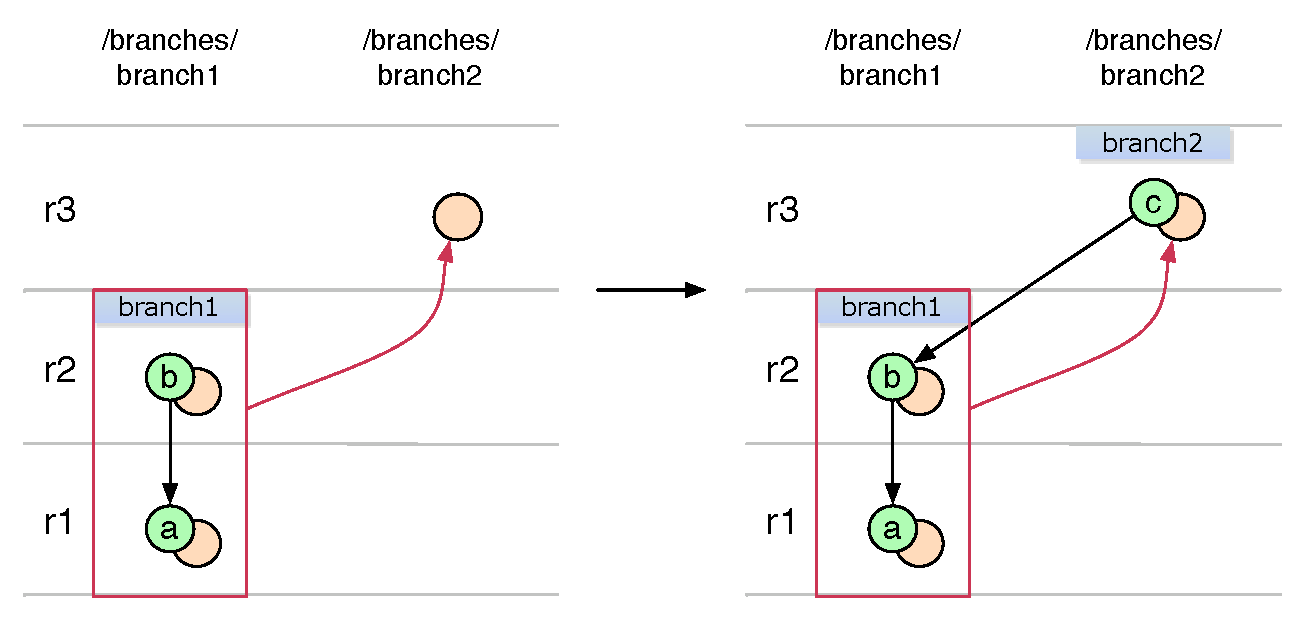
\includegraphics[width=\linewidth]{img/diagrams/branch_creation_from_mergeinfo_svn_to_git.pdf}
\caption{Subversion branch addition being translated to Git branch creation.}
\end{figure}

Subversion user at revision r3 added /branches/branch2 and set its mergehistory as /branches/branch1:r1-2. Translator will process revision r3 the way described at previous case.
\end{enumerate}

\subsubsection{Git Branch Creation}

\begin{enumerate}
\compactlist
\item Branch reference addition, figure \ref{git_branch_creation}.

\begin{figure}[!h]
\label{svn_branch_creation}
\centering
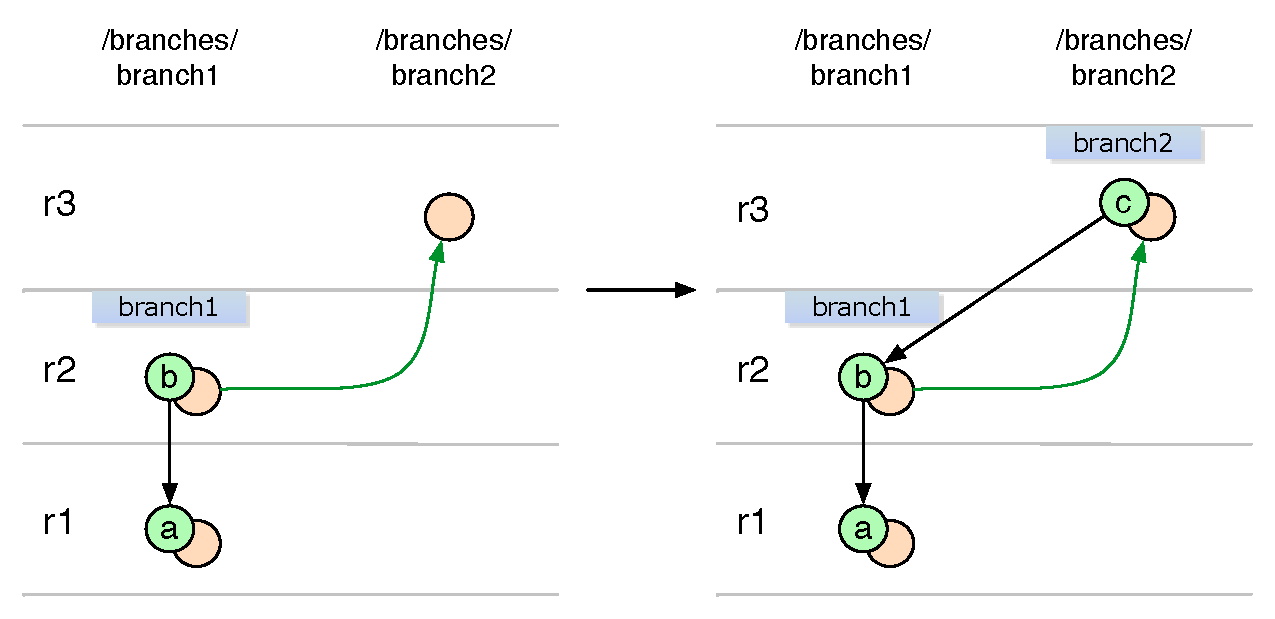
\includegraphics[width=\linewidth]{img/diagrams/branch_creation_svn_to_git.pdf}
\caption{Subversion branch copying being translated to Git branch creation.}
\end{figure}

Subversion user at revision r3 copied /branches/branch1@r2 to /branches/branch2. For that change Translator creates commit with:
\begin{itemize}
	\item Tree Object corresponding to /branches/branch2 subdirectory contents
	\item Author Ident and Committer Ident corresponding to the author of the revision
	\item Date of the revision
	\item Commit message of the revision
	\item Parent commit \emph{b}
\end{itemize}
And finally Translator adds /refs/heads/branch2 reference to the created commit \emph{c}.

% end of item
\item Addition with merge history. See \ref{svn_branch_creation_from_mergeinfo}.

\begin{figure}[!h]
\label{svn_branch_creation_from_mergeinfo}
\centering
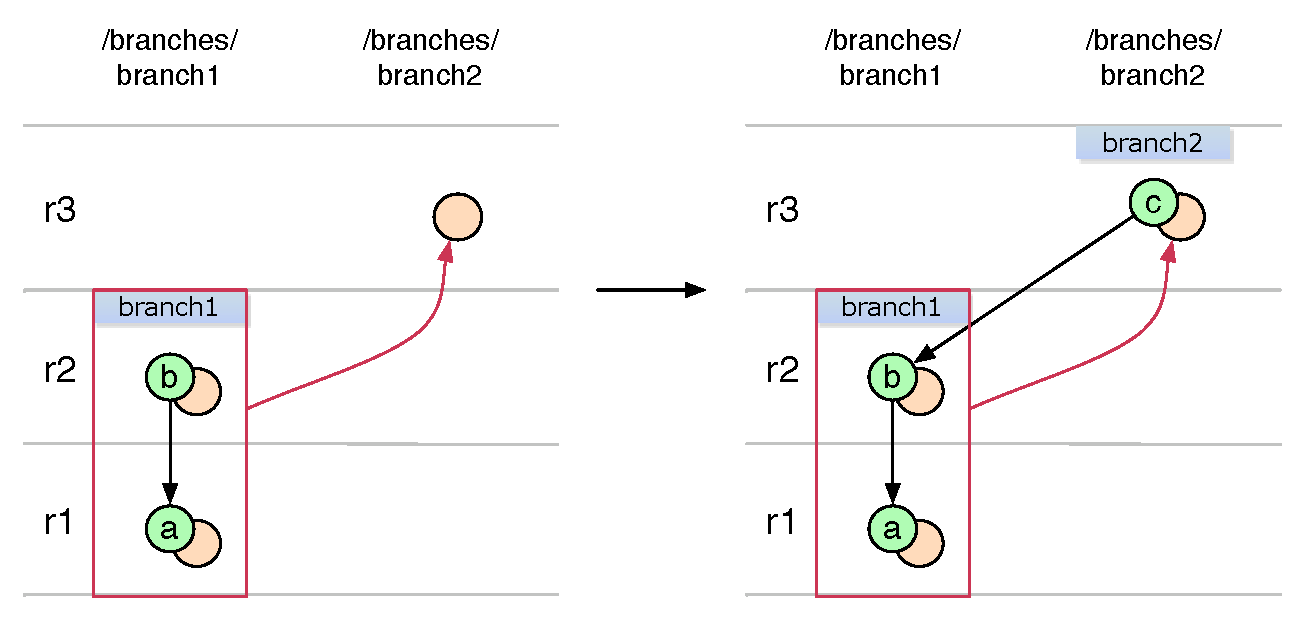
\includegraphics[width=\linewidth]{img/diagrams/branch_creation_from_mergeinfo_svn_to_git.pdf}
\caption{Subversion branch addition being translated to Git branch creation.}
\end{figure}

Subversion user at revision r3 added /branches/branch2 and set its mergehistory as /branches/branch1:r1-2. Translator will process revision r3 the way described at previous case.
\end{enumerate}
